%!TEX TS-program = pdflatex
%!TEX root = tesi.tex
%!TEX encoding = UTF-8 Unicode

\chapter{Risultati Ottenuti}
\todo[inline]{sommario capitolo}
% descrizione architettura migliore e a chi ci siamo ispirati N.R.
\todo[inline]
{
  Preambolo sulla accuratezza dei modelli creati
  Problema dell'AE perché non fornisce accuratezza, come parametro di valutazione si è utilizzata la loss
  La loss non poteva essere usata come discrtiminatoe perché troppo poco sensibile all'errore di presenza-nonpreseena della colla
  Un altro criterio di valutazione era una verifica a mano della qualità della differenza conforme in out

  Descrivere architettura migliore
  Descrivere post-processing a valle
}

\section{Il nostro obbiettivo TODO}
In figura~\ref{fig:obbiettivo_in_out_diff} sono riportate tre immagini per chiarire in che modo gli \textit{autoencoder} sono stati sfruttati per classificare Conformi e Scarti.
La figura~\ref{fig:obbiettivo_in} illustra uno Scarto.
L'immagine riportata in figura~\ref{fig:obbiettivo_out} è quella che si vorrebbe ottenere dall'AE a partire dallo Scarto appena illustrato.
Notare come si vorrebbe che il pezzo fosse riprodotto il più fedelmente possibile, ma che l'informazione della colla venisse rimossa.
In questo modo sarebbe possibile effettuare una differenza \textit{pixel} per \textit{pixel} tra immagine in ingresso ed immagine in uscita (detta anche ricostruita) ottenendo così un risultato simile a quello in figura~\ref{fig:obbiettivo_diff}.

Nel caso migliore possibile la classificazione verrebbe effettuata verificando se nell'immagine differenza tutti i valori sono zero.
Ossia l'immagine in ingresso appartiene alla classe Conforme ed è stata ricostruito alla perfezione.
Dato che ci si aspetta che l'\textit{autoencoder} non ricostruisca la colla nell'immagine in uscita, nell'immagine differenza ci sarà un'area di \textit{pixel} con valori in assoluto maggiori di zero.

È impossibile che l'\textit{autoencoder} raggiunga una precisione così alta, infatti è molto più infatti che l'immagine ricostruita sia soltanto un'approssimazione dell'immagine in ingresso.
Si ricorda che molto probabilmente l'AE rimuoverà tutte quelle caratteristiche particolari di un pezzo (graffi, macchie, \dots ), perché sono rumore rispetto ad una carcassa media.

Quindi si può affermare che la classificazione è divisa in due parti: nella prima l'immagine viene elaborata dall'\textit{autoencoder}; nella seconda l'immagine in ingresso e quella in uscita vengono confrontate, questa parte prende il nome di \textit{post-processing}.
L'effettiva classificazione viene eseguita in quest'ultima parte.

\begin{figure}[ht] % TODO
  \begin{center}
    \begin{tabular}{ccc}

      \begin{subfigure}{.3\linewidth}
        \centering\includegraphics[width=\textwidth]{example-image}
        \caption{Immagine in ingresso}
        \label{fig:obbiettivo_in}
      \end{subfigure} &

      \begin{subfigure}{.3\linewidth}
        \centering\includegraphics[width=\textwidth]{example-image}
        \caption{Immagine ricostruita}
        \label{fig:obbiettivo_out}
      \end{subfigure} &

      \begin{subfigure}{.3\linewidth}
        \centering\includegraphics[width=\textwidth]{example-image}
        \caption{Immagine differenza}
        \label{fig:obbiettivo_diff}
      \end{subfigure}

    \end{tabular}
    \caption{TODO in out diff}
    \label{fig:obbiettivo_in_out_diff}
  \end{center}
\end{figure}

\section{Metriche di valutazione}
Definire delle metriche per stabilire quali architetture preformassero meglio è stata una parte critica.
Infatti gli \textit{autoencoder} potevano essere confrontati solo tramite due criteri: uno numerico, ossia la \textit{MSE Loss} ottenuta durante l'allenamento, ed uno qualitativo, cioè osservare la qualità generale delle immagini generate.
Purtroppo nessuna delle due metriche permette di ottenere delle percentuali esatte sull'accuratezza delle classificazioni.
Tali dati numerici sono stati ottenuti soltanto quando le immagini differenza sono risultate soddisfacenti e si è quindi potuto sviluppare l'algoritmo di \textit{post-processing}.
\todo{c'è da dire altro?}


\section{Il modello}
L'architettura illustrata in figura~\ref{fig:ae16_arch}\footnote{L'immagine è stata generata usando \url{https://github.com/HarisIqbal88/PlotNeuralNet}} ha dato i risultati migliori. % TODO dire meglio
Elenchiamo le sue caratteristiche principali:
\begin{itemize}
  \item l'immagine in ingresso è in scala di grigi e di lato $200$ \textit{pixel};

  \item ogni strato convolutivo o convolutivo trasposto ha filtri di dimensione $5$x$5$, ha \textit{stride} pari a $1$, non ha nessun \textit{padding} e tutti (tranne il primo e l'ultimo strato) hanno $ch_{in}=ch_{out}=32$.
    %Il primo strato ha un canale ingresso, dato che l'\textit{input} non è a colori,
    Inoltre tutti i \textit{layer} utilizzano la funzione di attivazione \textit{ReLU}, fatta eccezione per l'ultimo in cui è presente la funzione sigmoidea.
    Infatti le immagini, prima di essere passate alla rete, vengono normalizzate in $[0,1]$, cioè facilita i calcoli effettuati all'interno dell'\textit{autoencoder}.
    L'output della rete, appartenente a $[0,1]$, verrà mappato nuovamente nell'intervallo $[0,255]$.

  \item tutti i \textit{max-pool layer} hanno sia il filtro che il passo pari a 2;

  \item il primo strato denso prende un vettore di $24*24*32=18432$ valori e lo mappa in uno spazio $2000$-dimensionale.
    Questa corrisponde alla massima compressione dell'informazione;

  \item il secondo strato denso effettua l'operazione opposta, mappando il vettore dello spazio latente in uno che possa avere le dimensioni di $24*24*32$.

\end{itemize}
%TODO fare tabella con i parametri di ogni strato?
Complessivamente la rete deve imparare  $73 832 000$ parametri.
Di questi metà si trovano nell'\textit{encoder} e metà nel \textit{decoder}.
Questo valore potrebbe sembrare grande ma, osservando che la VGG11~\cite{vgg} ha più di 130 milioni di parametri, risulta ragionevole.
Si fa notare che la maggior parte dei parametri è contenuto nei due strati densi.
Sappiamo che il numero di parametri di uno strato è dato da $n * m$ con $n$ ed $m$le dimensioni dei vettori in ingresso ed in uscita.
Nel nostro caso abbiamo due strati da $18432 * 2000 = 36 864 000$ parametri l'uno.
I quattro \textit{layer} convolutivi e convolutivi trasposti da 32 canali in ingresso ed in uscita hanno $25600$ parametri ciascuno.
\todo[noline]{cos'altro da dire?}

\begin{figure}[ht]
  \begin{center}
    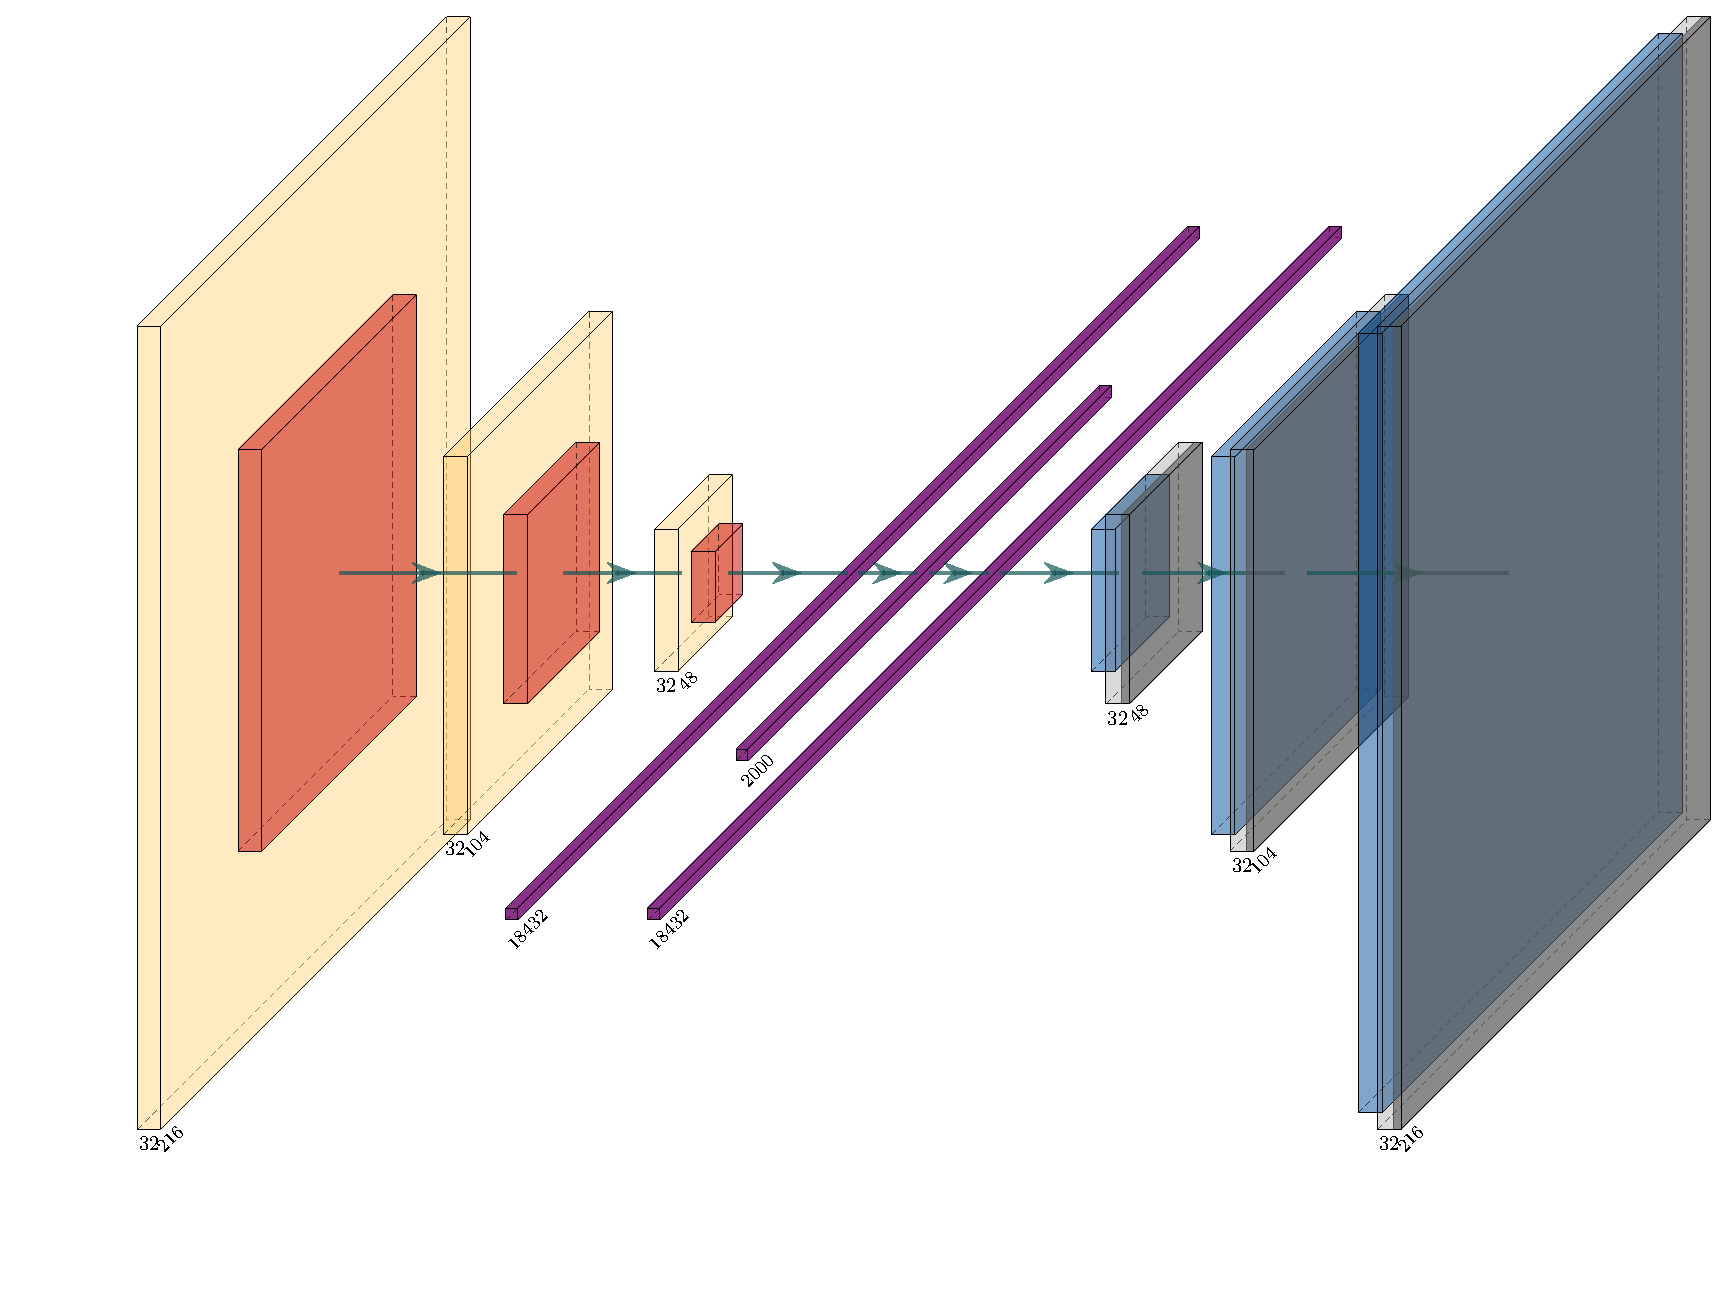
\includegraphics[width=.9\textwidth]{ae16}
    \caption{TODO architettura della rete}
    \label{fig:ae16_arch}
  \end{center}
\end{figure}
\todo{rifai disegno architettura i conv trans sono svaccati}

L'allenamento del modello in figura~\ref{fig:ae16_arch} è stato effettuato sui Conformi del \textit{dataset}, processati come descritto a pagina~\pageref{prep} e seguenti.
In questa fase non sono stati utilizzati né gli Scarti né gli Scarti Sintetici.

Durante l'allenamento si è utilizzata la \textit{MSE Loss} confrontando lo Scarto tra l'immagine in ingresso e l'immagine ricostruita.
Nel grafico in figura~\ref{fig:loss_plot} si può notare come la \textit{loss} scenda in modo repentino nelle prime 5 epoche per poi stabilizzarsi.
Il tasso di apprendimento\footnote{In inglese \textit{learning rate}} è stato gestito dinamicamente: se al passare delle epoche la \textit{loss} non è calata, allora il tasso di apprendimento viene diviso per un fattore dieci.

\begin{figure}[ht] % TODO sarebbe da cambiare
  \begin{center}
    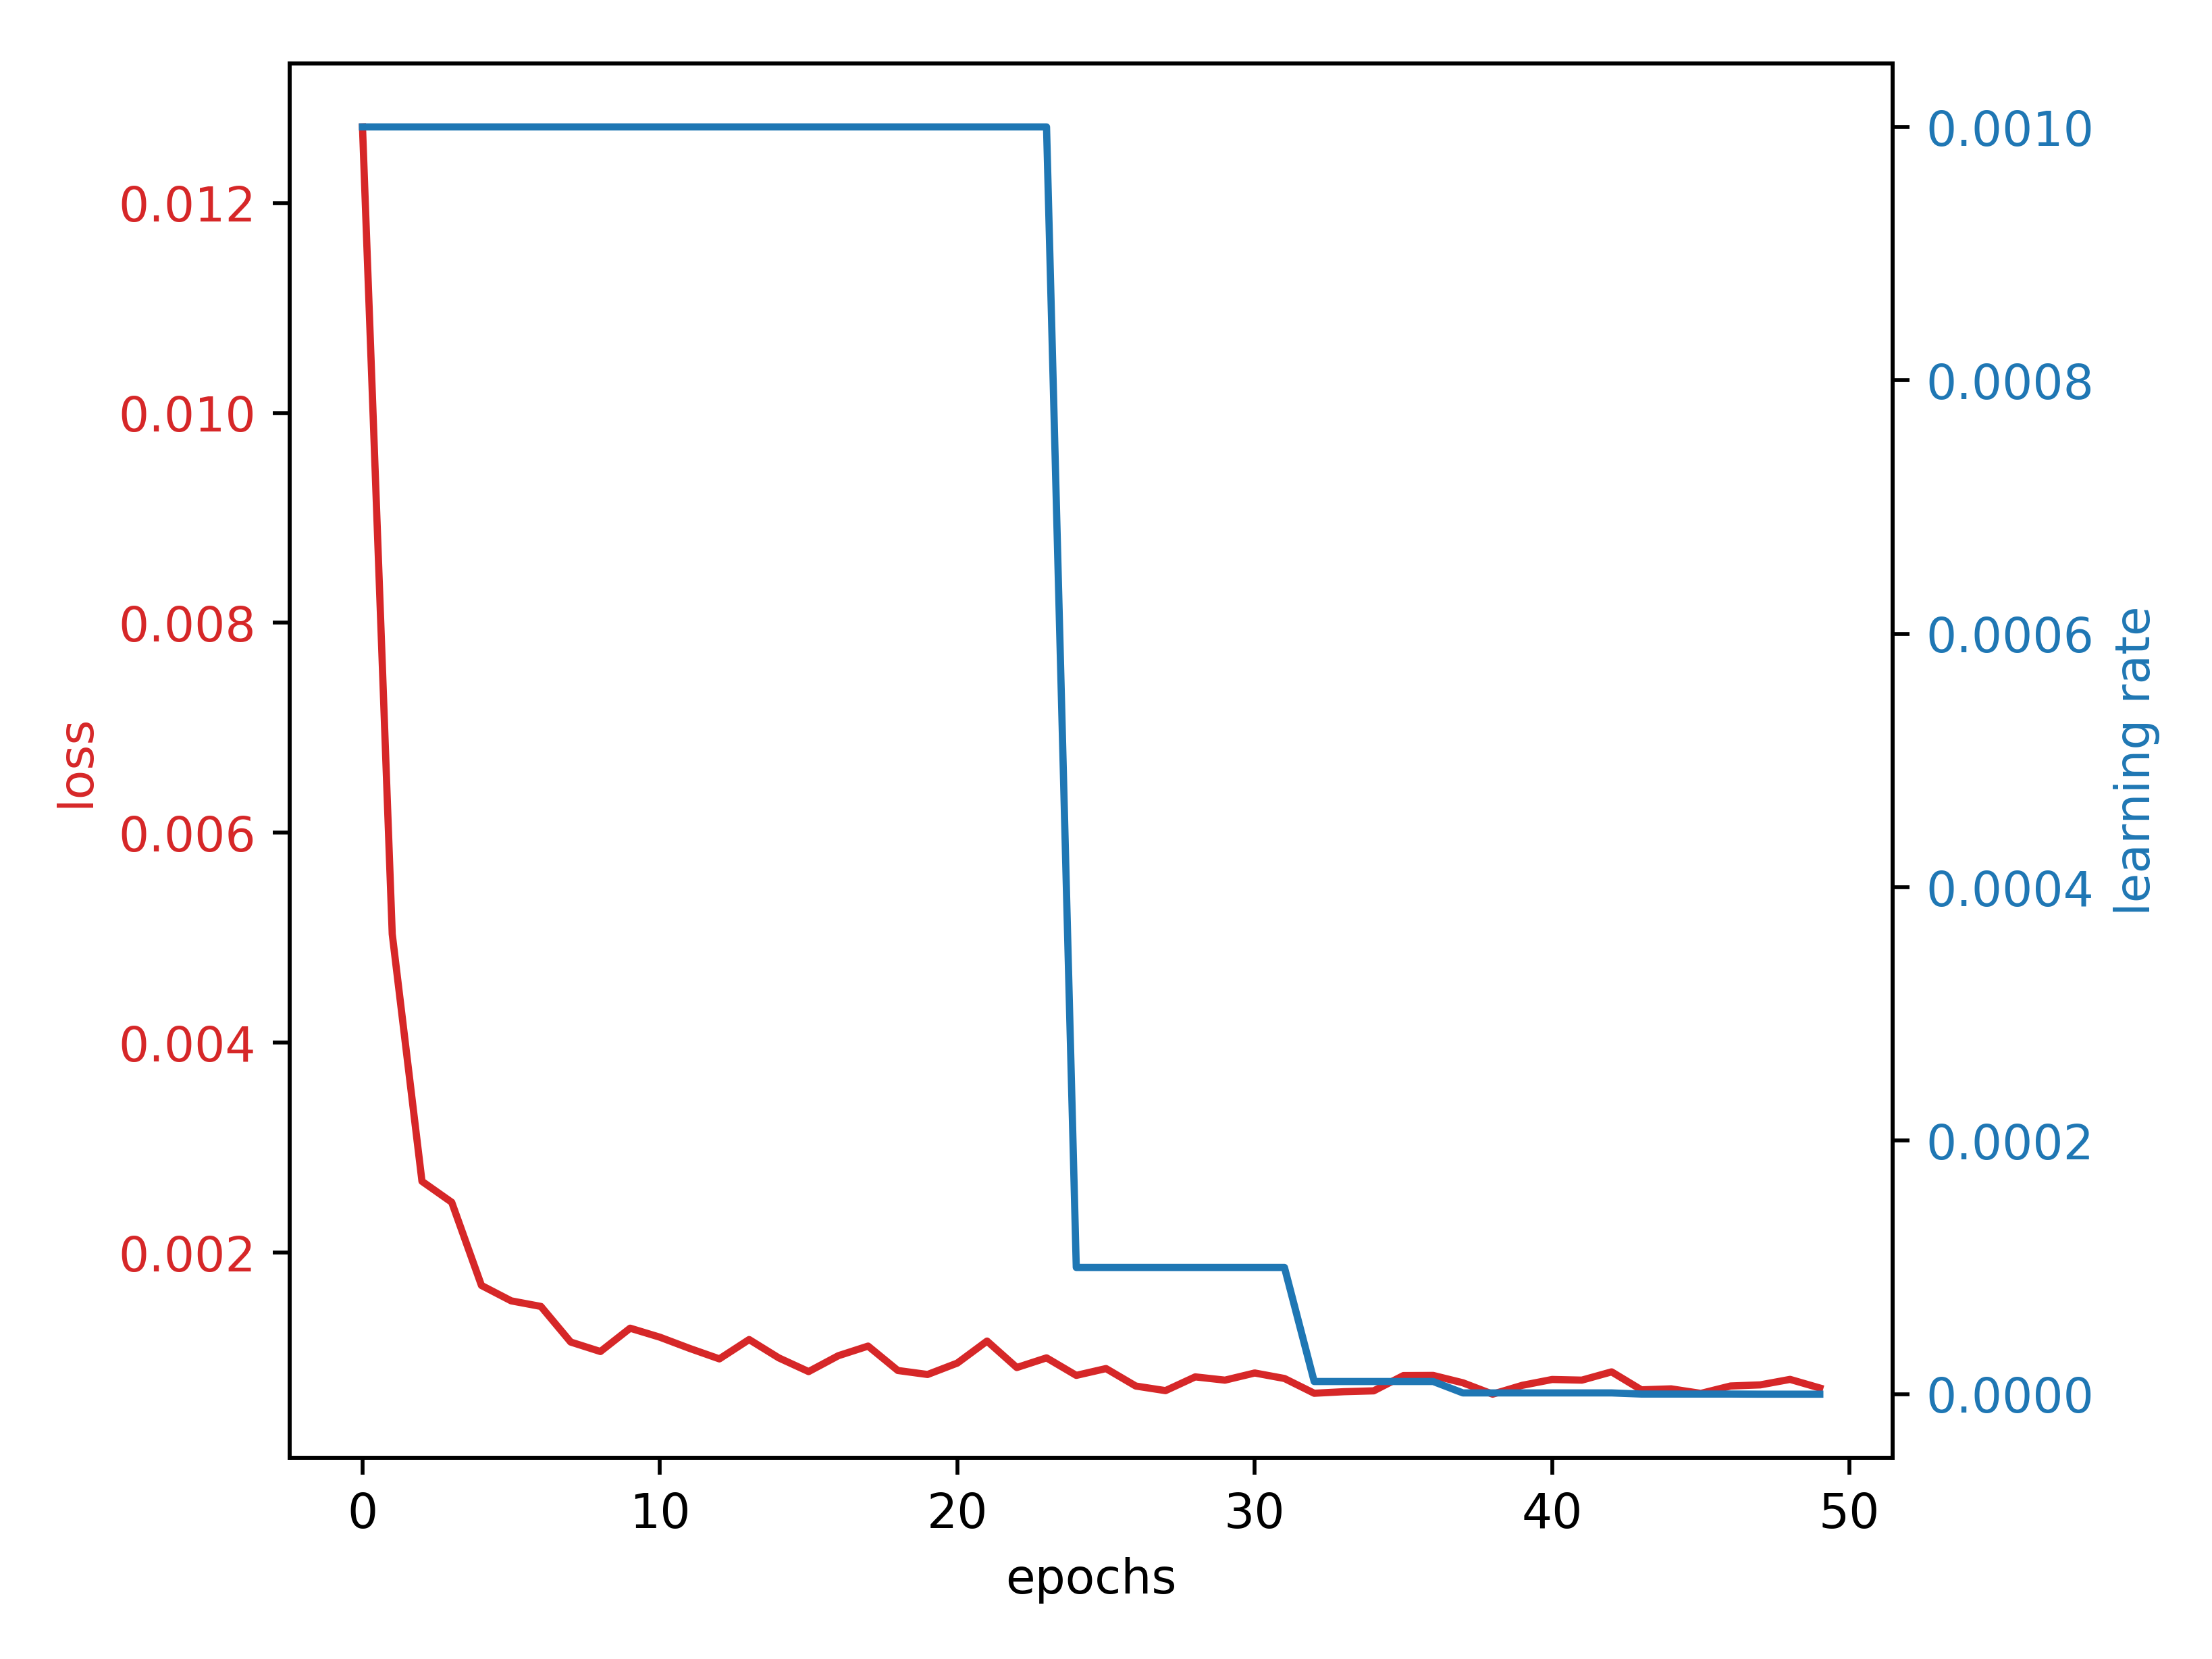
\includegraphics[width=0.5\textwidth]{loss_plot}
    \caption{Andamento della \textit{loss} e del \textit{learning rate} al passare delle epoche}
    \label{fig:loss_plot}
  \end{center}
\end{figure}

Ogni cinque epoche è stata generata un'immagine con alcuni Conformi in ingresso  ed in uscita.
È interessante notare, osservando figura~\ref{fig:epoch_0}, come le prime ricostruzioni siano tutte uguali.
Nella figura sono riportati, in alto, i sei esemplari dati in \textit{input} alla rete, mentre in basso sono mostrate le loro ricostruzioni.
Probabilmente questo è dovuto al fatto che i pesi si distribuiscono fin da subito in modo da catturare le proprietà comuni a tutte le immagini, ad esempio l'area nera della maschera e gli anelli concentrici.
In figura~\ref{fig:epoch_45} è riportato un altro gruppo di Conformi assieme alle ricostruzioni relative all'epoca numero quarantacinque.
Ci si accorge subito che le immagini in uscita risultano meno sgranate e che in alcune di esse sono state generate perfino macchie ed aree più scure.
Come ci si poteva aspettare la superficie delle immagini in \textit{output} risulta molto più lisca e priva della maggior parte dei graffi.

\begin{figure}[ht] % TODO sarebbe da cambiare
  \begin{center}
    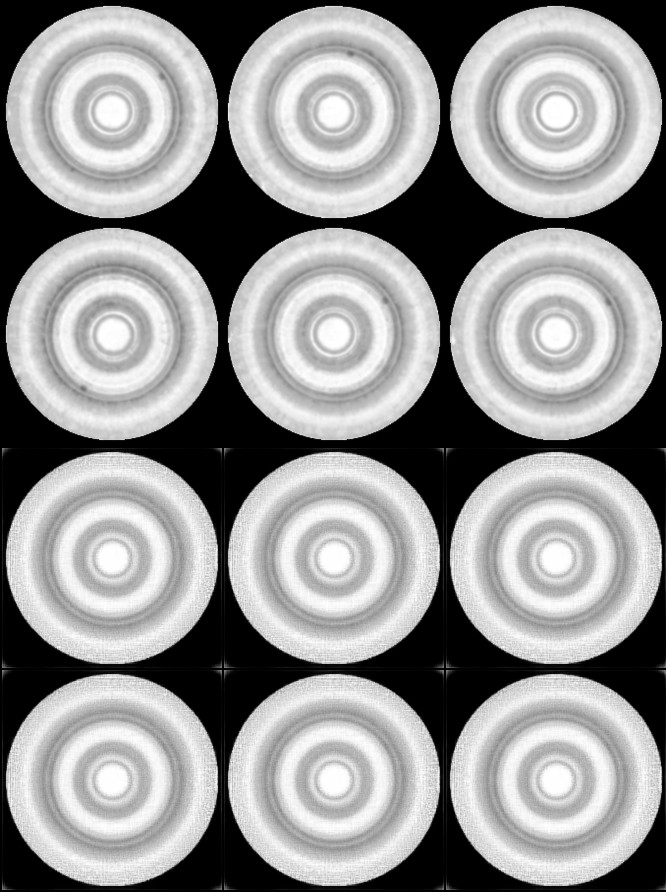
\includegraphics[width=.65\textwidth]{in_out_epoch_0}
    \caption{In alto 6 immagini Conformi in \textit{input}, in basso la loro ricostruzione alla prima epoca}
    \label{fig:epoch_0}
  \end{center}
\end{figure}

\begin{figure}[ht] % TODO sarebbe da cambiare
  \begin{center}
    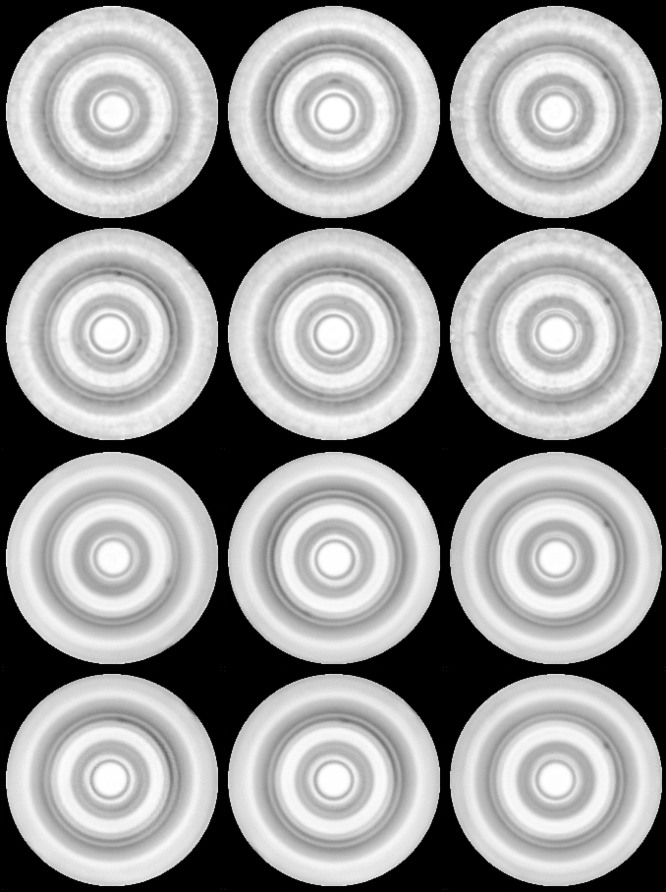
\includegraphics[width=.65\textwidth]{in_out_epoch_45}
    \caption{In alto 6 immagini Conformi in \textit{input}, in basso la loro ricostruzione alla 45-esima epoca}
    \label{fig:epoch_45}
  \end{center}
\end{figure}

\clearpage
\section{Post-Processing}
Dopo aver osservato la precisione con cui i Conformi vengono riprodotti bisogna verificare come l'AE si comporti con le immagini della classe Scarto.
In figura~\ref{fig:scarti_in_out} si possono osservare alcuni esempi di Scarti all'ingresso e all'uscita dell'\textit{autoencoder}.
Notare come nelle prima coppia la colla sia stata rimossa molto bene e la carcassa ricostruita abbia alcune caratteristiche di quella originale.
Purtroppo nell'ultima coppia si vede come le zone più scure tipiche di alcune carcasse con colla, causino la creazione di rumore nell'immagine in \textit{output}.
Proprio questo motivo ha portato alla creazione degli Scarti Sintetici.
Si fa subito presente che gli Scarti Sintetici sono stati generati a partire da un gruppo di Conformi differente dall'insieme di immagini usate durante l'allenamento.

\begin{figure}[ht] % TODO
  \begin{center}
    \begin{tabular}{c}

      %\begin{subfigure}{\linewidth}
      %  \begin{center}
      %    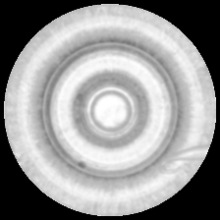
\includegraphics[width=.3\textwidth]{128___1315_1_0_1_OnLineAnalysis_in}
      %    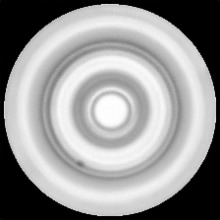
\includegraphics[width=.3\textwidth]{128___1315_1_0_1_OnLineAnalysis_out}
      %  \end{center}
      %\end{subfigure} \\ \\

      %\begin{subfigure}{\linewidth}
      %  \begin{center}
      %    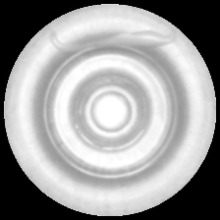
\includegraphics[width=.3\textwidth]{128___14147_1_0_1_OnLineAnalysis_in}
      %    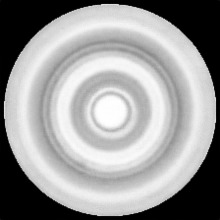
\includegraphics[width=.3\textwidth]{128___14147_1_0_1_OnLineAnalysis_out}
      %  \end{center}
      %\end{subfigure} \\ \\

      \begin{subfigure}{\linewidth}
        \begin{center}
          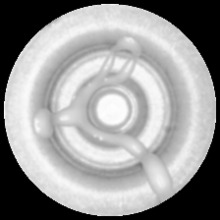
\includegraphics[width=.3\textwidth]{128___22886_1_1_1_OnLineAnalysis_in}
          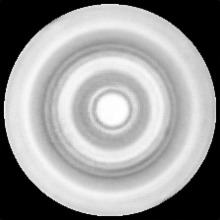
\includegraphics[width=.3\textwidth]{128___22886_1_1_1_OnLineAnalysis_out}
        \end{center}
      \end{subfigure} \\ \\

      \begin{subfigure}{\linewidth}
        \begin{center}
          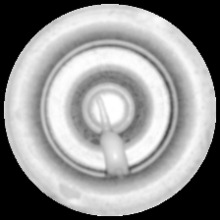
\includegraphics[width=.3\textwidth]{128___33667_0_0_1_OnLineAnalysis_in}
          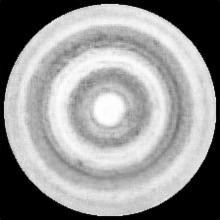
\includegraphics[width=.3\textwidth]{128___33667_0_0_1_OnLineAnalysis_out}
        \end{center}
      \end{subfigure}

    \end{tabular}
    \caption{Esempi di Scarti e loro ricostruzione}
    \label{fig:scarti_in_out}
  \end{center}
\end{figure}

L'algoritmo di post-processing è stato sviluppato usando immagini differenza generate da Scarti Sintetici, perché risultano più pulite.
Ma soprattutto perché ci si aspetta che siano anche più verosimili a quelle che si otterrebbero durante la messa in opera del sistema: le carcasse sono state scelte dalla distribuzione dei Conformi. \todo{dire meglio o non dire affatto}

In figura~\ref{fig:post_proc_scarto_sin} si possono vedere l'immagine di partenza (in alto a sinistra), l'immagine ricostruita dall'\textit{autoencoder} (in alto a destra), il risultato del post-processing della differenza fra le due (in basso a destra) e la predizione finale.
L'algoritmo di \textit{post-processing}, ottenuto con metodi empirici, opera in questo modo:
\begin{itemize}
  \item viene calcolato il valore assoluto della differenza \textit{pixel} per \textit{pixel} tra le immagini d'\textit{input} e d'\textit{output}.
    Il risultato di questo passaggio non è stato mostrato perché i valori non sono molto grandi, ciò significa che l'immagine, principalmente nera, contiene alcune aree con \textit{pixel} di colore grigio scuro;

  \item viene effettuata una doppia sogliatura sull'immagine differenza.
    In questo modo tutti i pixel con valori sufficientemente grandi vengono ricolorati di bianco, mentre i restanti sono mappati a $0$;

  %\item viene applicato un filtro che rimuove tutti i \textit{pixel} isolati o che compongono un gruppo troppo piccolo TODO in caso estendere...

  \item viene utilizzato un algoritmo di rilevamento di macchie che sfrutta la differenza di gaussiane.
    Si effettuano varie convoluzioni con filtro di Gauss, in questo modo le macchie più piccole verranno sfumate sempre più fino a scomparire.
    Effettuando differenze tra immagini più o meno sfumate si può determinare se la macchia ha dimensioni sufficientemente grandi e stimarne il centro;
  %https://en.wikipedia.org/wiki/Difference_of_Gaussians

\end{itemize}

Si è verificato che questo tipo di manipolazione non generasse falsi positivi: i valori delle soglie e la dimensione minima delle macchie che si rilevano sono tali da rimuovere il rumore delle immagini differenza.

Va detto che molti Scarti vengono predetti come tali anche a causa delle fasce più scure, che non permettono una ricostruzione fedele  della carcassa oppure risultano grandi a sufficienza nell'immagine differenza.

\begin{figure}[ht] % TODO
  \begin{center}
    \begin{tabular}{cc}

      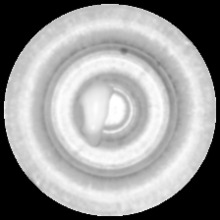
\includegraphics[width=.3\textwidth]{128___17299_0_1_1_OnLineAnalysis_con_colla_in} &
      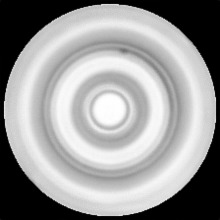
\includegraphics[width=.3\textwidth]{128___17299_0_1_1_OnLineAnalysis_con_colla_out} \\
      %
\includegraphics[width=.3\textwidth]{128___17299_0_1_1_OnLineAnalysis_con_colla_diff} & 
      
\includegraphics[width=.3\textwidth]{128___17299_0_1_1_OnLineAnalysis_con_colla_to_blob} &
      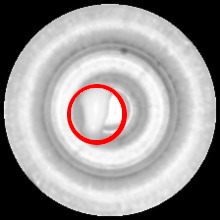
\includegraphics[width=.3\textwidth]{128___17299_0_1_1_OnLineAnalysis_con_colla_detected}

    \end{tabular}
    \caption{Post-processing applicato ad uno Scarto Sintetico}
    \label{fig:post_proc_scarto_sin}
  \end{center}
\end{figure}

\clearpage
\section{I Risultati}
Riassumiamo ora brevemente i risultati ottenuti.
Come si vede nella tabella~\ref{tab:test_predicions}, tutti i Conformi (che non sono stati usati durante l'allenamento) sono stati classificati correttamente.
Viceversa non tutti gli Scarti e gli Scarti Sintetici sono stati classificati come tali.
Per quanto riguarda i secondi va specificato che sono stati scelti a caso trenta Conformi e su ciascuno è stato applicato un ritaglio di colla.
Osservando gli elementi predetti in modo scorretto e la relativa immagine differenza ci si accorge che la colla può passare inosservata se:
\begin{itemize}
  \item ha un colore molto vicino a quello della superficie della carcassa, quindi tende a corrispondere, nell'immagine differenza, ad un area con valori in assoluto piccoli;
  \item si presenta come una striscia sottile.
\end{itemize}

\begin{table}[ht]
  \centering
  \begin{tabular}{||l r r r||}
    \hline
    %\multicolumn{4}{||c||}{tittolo} \\ \hline
    Classe           & Elementi & Predetti come KO & Percentuale \\ \hline \hline
    Conformi         & 314      & 0                & 0\%         \\ \hline
    Scarti           & 30       & 28               & 93.3\%      \\ \hline
    Scarti Sintetici & 30       & 28               & 93.3\%      \\ \hline

  \end{tabular}
  \caption{Predizioni sull'insieme di \textit{Test}}
  \label{tab:test_predicions}
\end{table}

Questi dati sono riportati anche sotto forma di matrice di confusione in tabella~\ref{tab:confusion_matrix}.
Possiamo usare la tabella per ricavare le metriche di \textit{accuracy}, \textit{precision} e \textit{recall} definite come:
\begin{align*} % TODO allineare
  accuracy &= \frac{\text{TP + TN}}{\text{TP + TN + FP + FN}}
            = \frac{56 + 314}{56 + 314 + 4} = 0.989
  \\ \\
  precison &= \frac{\text{TP}}{\text{TP + FP}} 
            = \frac{56}{56} = 1.00
  \\ \\
  recall   &= \frac{\text{TP}}{\text{TP + FN}} 
            = \frac{56}{56 + 4} = 0.933
\end{align*}
Notiamo come la \textit{accuracy}, che indica quante volte viene predetta la classe corretta, sia molto alta.
Non ci sorprende che la \textit{precision} sia così alta perché uno dei nostri obbiettivi era evitare che venissero scartati Conformi.
Quindi si voleva mantenere il numero di Falsi Positivi il più basso possibile.
Il valore più basso è la \textit{recall} ossia che percentuale degli Scarti è stati effettivamente riconosciuta, valore comunque soddisfacente perché corrisponde al 93.3\%.

\begin{table}[ht]
  \centering
  \renewcommand\arraystretch{1.5}
  \setlength\tabcolsep{0pt}
  \begin{tabular}{c >{\bfseries}r @{\hspace{0.7em}}c @{\hspace{0.4em}}c @{\hspace{0.7em}}l}
    \multirow{10}{*}{\parbox{1.1cm}{\bfseries\raggedleft Valore\\ effettivo}} & 
      & \multicolumn{2}{c}{\bfseries Predizione} & \\
    & & \bfseries 60 & \bfseries 314 & \bfseries totale \\
    & p$'$ & \MyBox{56 TP}{} & \MyBox{4 FN}{} & 60 \\[2.4em]
    & n$'$ & \MyBox{0 FP}{} & \MyBox{314 TN}{} & 314 \\
    & totale & 56 & 318 &
  \end{tabular}
  \caption{Matrice di confusione per l'insieme di \textit{Test}}
  \label{tab:confusion_matrix}
\end{table}

Per avere una stima sulle capacità della rete su un numero maggiore di Conformi si è deciso di effettuare delle predizioni anche sulle immagini usate durante l'allenamento.
Generalmente le immagini differenza della carcasse Conformi si presentano quasi interamente nere.
Le poche macchie bianche sono di dimensioni ridotte e distanti tra loro.
Il principale motivo che causa una predizione errata è il fatto che il pezzo sia stato fotografato da una distanza maggiore della media.
Questo significa che le balze non vengono coperte interamente dalla maschera e quindi, dato che l'AE non le può ricostruire, possono risultare come una macchia sufficientemente grande.
Nella tabella~\ref{tab:train_predicions} viene illustrato che il 98.9\% dei Conformi viene identificato correttamente.

\begin{table}[ht]
  \centering
  \begin{tabular}{||l r r r||}
    \hline
    Classe           & Elementi & Predetti come KO & Percentuale \\ \hline \hline
    Conformi         & 1375     & 15               & 1.1\%       \\ \hline

  \end{tabular}
  \caption{Predizioni sull'insieme di \textit{Train}}
  \label{tab:train_predicions}
\end{table}

